250. \begin{figure}[ht!]
\center{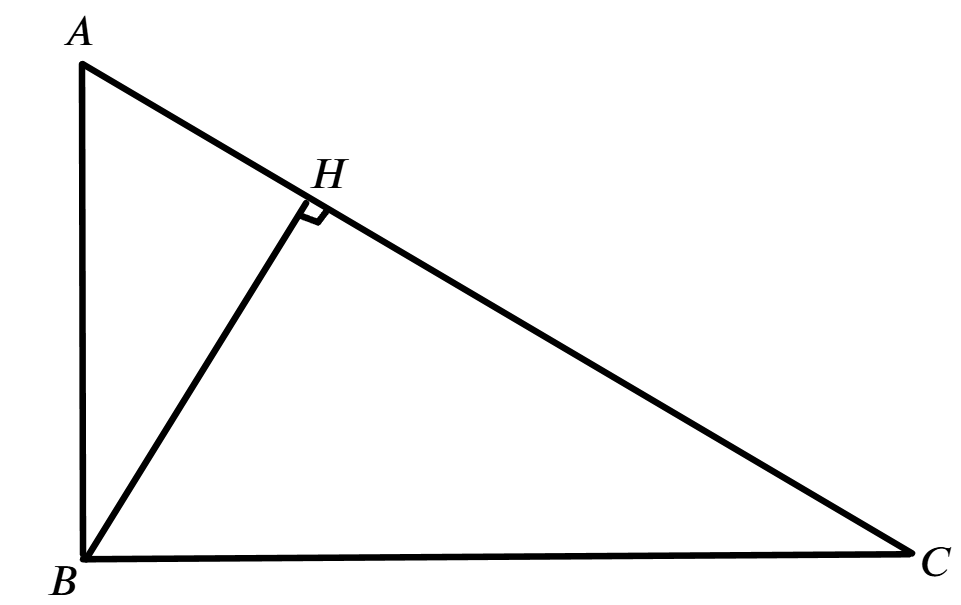
\includegraphics[scale=0.35]{g8-245.png}}
\end{figure}\\
Так как квадрат высоты, проведённой из прямого угла, равен произведению отрезков, на которые она делит гипотенузу, имеем соотношение $BH^2=(BH-3)(BH+4),\ BH^2=BH^2+4BH-3BH-12,\ BH=12$см. Тогда по теореме Пифагора найдём катеты:
$AB=\sqrt{144+81}=15$см и $BC=\sqrt{144+256}=20$см.
ewpage
oindent
